\noindent \\
\section{Logs}\label{sec:logs-processing}

Treballarem els registres d'accés a la plataforma d'UPCommons.
Ens han proporcionat aquestes dades que corresponen als accessos des de del primer dia de l'any 2006 fins al darrer dia del 2023.

\clearpage

\subsection{Anàlisi superficial dels \textit{\gls{log}s}}\label{subsec:log-analysis}

El format dels fitxers d'entrada on hi són emmagatzemats els registres és d'un text pla on es registren tots els \textit{\gls{log}s} corresponents a un dia.
Tractant-se de la informació d'accés als recursos d'\gls{UPCommons}, accessibles des de la pàgina web,
tenim aquesta informació recollida des de la capa d'aplicació, mitjançant els missatges de petició del protocol \gls{HTTP}.

\begin{figure}[htbp]
    \centerline{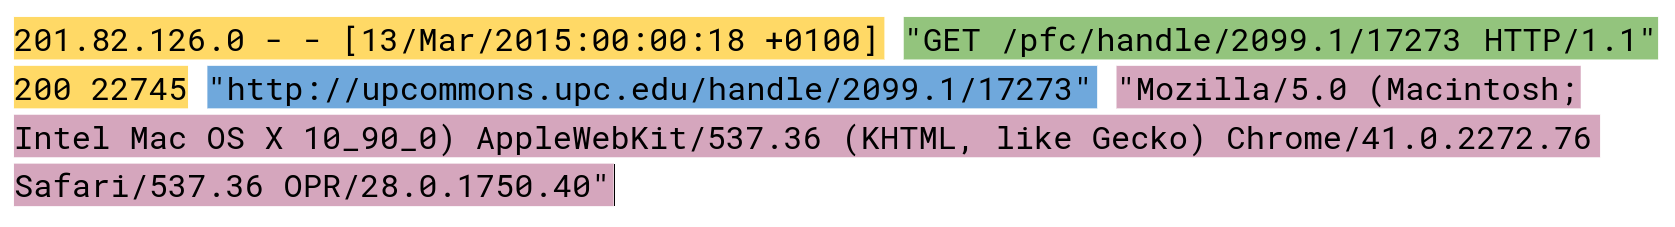
\includegraphics[width=1\textwidth]{figures/example-log}}
    \captionsetup{justification=centering}
    \caption{Exemple del contingut d'un \textit{\gls{log}}. (\textbf{Font}: \gls{UPCommons}.)}\label{fig:example-log}
\end{figure}


\noindent
Cada línia present als fitxers dels \textit{\gls{log}s} correspon a una petició \gls{HTTP} .
El format d'aquesta és el següent:

\noindent \\
\textbf{Adreça \gls{IP}} \\ \\
Identificador de xarxa que indica l'agent que ha realitzat la petició.
L'agent pot ser:
\begin{itemize}
    \item Un usuari humà.
    \item Un agent automatitzat: robots, scripts, serveis de mail, etc.
\end{itemize}
Degut a qüestions de privacitat i protecció de dades, aquest identificador ha sigut modificat en un procés d'anonimització. \\

\begin{tcolorbox}[colback=green!5!white, colframe=green!50!black, title=Els usuaris poden estar darrera d'un NAT]\label{tcbox:iguals-emmascarats}
    No podem sempre afirmar que dues peticions amb el mateix identificador provenen del mateix usuari.
    Pot haver-hi darrere un \gls{NAT}, usuaris compartint dispositiu, etc.
\end{tcolorbox}

\noindent \\
\textbf{Data i hora} \\ \\
La marca temporal del registre ve definida per la seva data i hora.
Si bé es pot treballar directament amb aquest valor si segueix el format \gls{ISO}, és preferible utilitzar el format estàndard \gls{POSIX} (nombre de segons no intercalars des de l'1 de gener del 1970).
Aquest format és més simple, les comparacions són més eficients i evitem problemàtiques de diferències temporals en zones geogràfiques.

\clearpage

\noindent
\textbf{Informació de la petició \gls{HTTP}}~\cite{http} \\

\begin{itemize}
    \item Mètode de la petició: els més habituals són \texttt{GET}, \texttt{POST} i \texttt{HEAD} .
    \item Recurs accedit: enllaç al recurs accedit per la petició.
    \item Versió \gls{HTTP}: evolució d'\texttt{HTTP/1.0} fins a \texttt{HTTP/1.1} en el transcurs dels anys.
    No hi ha presència de registres amb \texttt{HTTP/2.0}.
    \item Codi d'estat que retorna la petició: codi que representa el resultat de la petició.
    Els més habituals són els \texttt{2XX} (succés), \texttt{3XX} (redireccions) \texttt{4XX} (error del client) i \texttt{5XX} (error del servidor)
    \item Mida de la resposta: mida en \textit{bytes} del cos de la resposta.
\end{itemize}

\noindent \\
\textbf{Referent} \\ \\
El camp del referent indica la ubicació d’on s’ha fet la sol·licitud del recurs accedit.

\noindent \\ \\
\textbf{User Agent} \\ \\
Amb l’ajuda d’aquest camp, podrem analitzar l’empremta digital del cercador utilitzat i determinar amb una certa precisió el tipus de dispositiu utilitzat, el sistema operatiu, si l’acció prové d’un usuari o d’una eina automatitzada (\textit{bots} o serveis de correu)

\clearpage

\subsection{Filtratge dels \textit{\gls{log}s}}\label{subsec:log-filter}

Un cop entenem l'estructura dels \textit{logs}, el següent pas és dur a terme un anàlisi preliminar del seu contingut.
Esmentarem diferents casos trobats durant el processament d'aquests. \\

\noindent
El cas principal és aquell \textit{\gls{log}} que incorpori informació sobre un accés a un recurs, o una cerca.
Els podrem identificar perquè:

\begin{itemize}
    \item Porten l’identificador \gls{handle}.
    \item Contenen referències a algun domini d’\gls{UPCommons}.
    \item En cas ser una cerca a la plataforma, porten l’etiqueta amb alguna paraula clau com \textit{discover}, \textit{browse} \dots
\end{itemize}

\noindent
Però els servidors registren \textbf{moltes} més coses.
És feina nostra decidir què fer en cada cas. \\

\noindent
\textbf{Accés a recursos web} \\ \\
Després d’un accés a algun recurs, generalment als \textit{\gls{log}s} es poden veure registres d’accessos a recursos web (en vermell),
com podrien ser fitxers \textit{css}, \textit{javascript}, \textit{gifs} \dots

\begin{figure}[htbp]
    \centerline{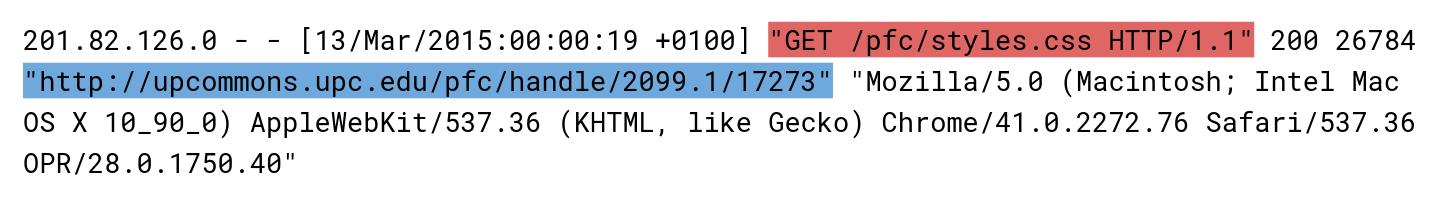
\includegraphics[width=\textwidth]{figures/log-web-resource}}
    \captionsetup{justification=centering}
    \caption{Exemple d'un \textit{\gls{log}} que accedeix a un recurs web, concretament una fulla d'estils \textit{\gls{CSS}} . (\textbf{Font}: \gls{UPCommons}.)}\label{fig:log-web-resource}
\end{figure}

\noindent \\
Com que aquests registres no ens aporten cap informació valuosa pels nostres casos d'ús, els \textbf{descartarem}.

\clearpage

\noindent
\textbf{Repeticions} \\

\noindent
Un \textit{\gls{log}} apareix exactament igual a diverses entrades, amb una petita diferèn-cia temporal (vermell).
Al següent exemple podem veure com el mateix accés es repeteix tres vegades (verd i groc), a diferents adreces \gls{IP} (vermell).

\begin{figure}[htbp]
    \centerline{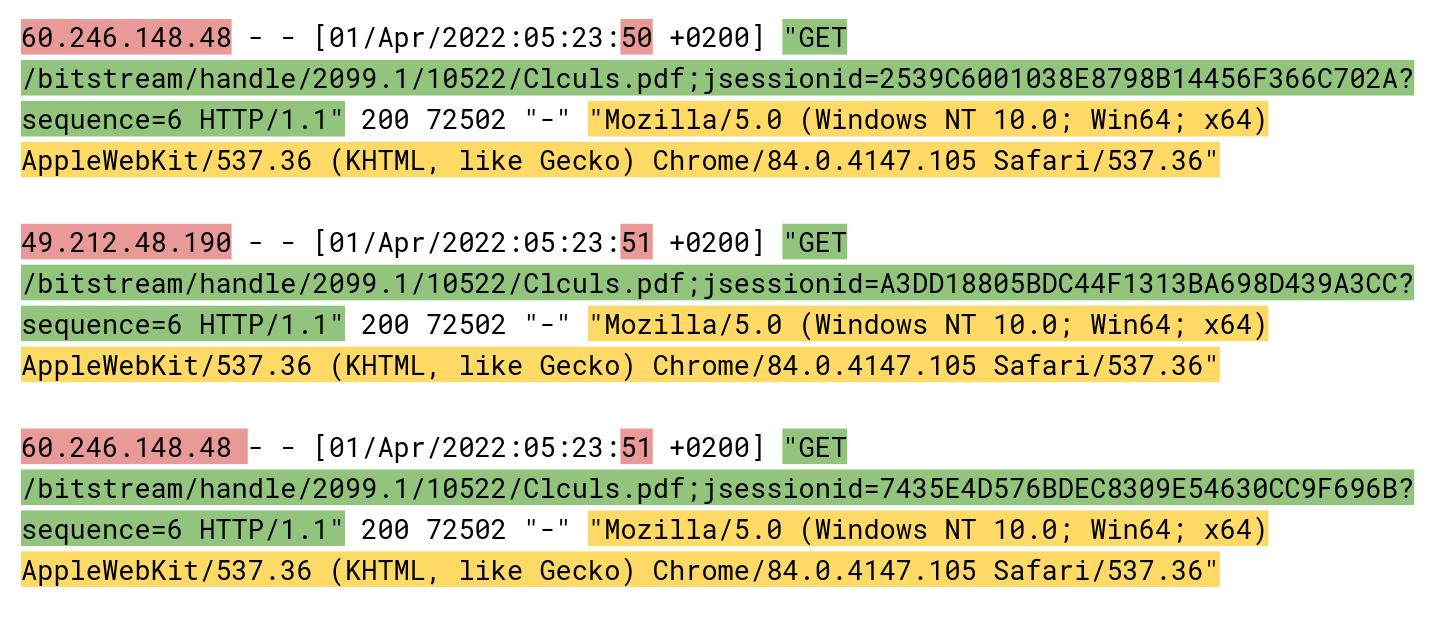
\includegraphics[width=\textwidth]{figures/log-repetitions}}
    \captionsetup{justification=centering}
    \caption{Exemple d'una cadena de \textit{\gls{log}s} que accedeixen al mateix contingut. (\textbf{Font}: \gls{UPCommons}.)}\label{fig:log-repetitions}
\end{figure}

\begin{tcolorbox}[colback=green!5!white, colframe=green!50!black, title=Divergència relativa]
    No podem sempre afirmar que peticions amb contingut igual, però diferents identificadors provenen d'usuaris diferents.
    Pot haver-hi darrere un servidor \textit{Proxy} que redirigeixi les peticions, distribuïdors de càrrega, etc.
    \tcblower
    Cas anàleg als ``iguals emmascarats''~\ref{tcbox:iguals-emmascarats}.
\end{tcolorbox}

\noindent
\begin{tcolorbox}[colback=blue!5!white, colframe=blue!75!black, title=Counter]
    Com a línia de treball futur, el projecte Counter~\cite{counter} pot servir com a base per tractar aquesta casuística.
\end{tcolorbox}

\noindent \\
Amb la finalitat d'enfocar l'anàlisi per altres bandes, no s'ha pres cap decisió en vers aquests casos, i seran tractats com la generalitat.

\clearpage

\noindent
\textbf{Cerques} \\

\noindent
Als \textit{\gls{log}s} hi són presents cerques dins de la plataforma \gls{UPCommons}. \\

\begin{figure}[htbp]
    \centerline{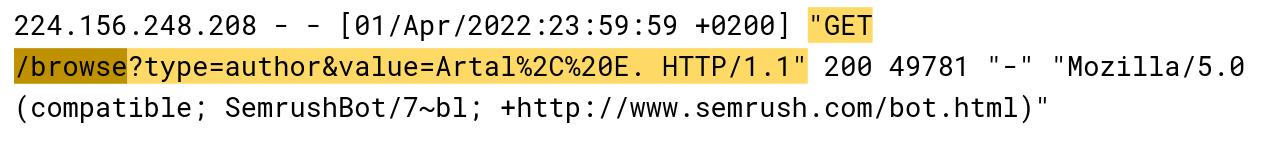
\includegraphics[width=\textwidth]{figures/log-search}}
    \captionsetup{justification=centering}
    \caption{Exemple d'un \textit{\gls{log}} d'una cerca a la plataforma. (\textbf{Font}: \gls{UPCommons}.)}\label{fig:log-search}
\end{figure}

\noindent
El procediment general no canvia respecta aquest cas.
Haurem de tenir en compte quins són, i diferenciar-los de la resta. \\

\noindent
\textbf{Errors de processament}\label{subsubsection:log-errors} \\

\noindent
Diem que un \textit{\gls{log}} produeix un error de processament si el seu format difereix abruptament del general (vegeu ~\ref{subsec:log-analysis}).
Diferenciarem entre dos casos:

\begin{itemize}
    \item \textbf{Errors reversibles:} són aquells que segueixen un paradigma.
    La seva presència és abundant.
    Alguns exemples śon:
    \begin{itemize}
        \item L'adreça \gls{IP} no existeix o és mal formada.
        \item Contingut alterat (a vegades, intencionadament!)
    \end{itemize}
    En aquests casos manipularem el registre afectat per homogeneïtzar el conjunt dels \textit{logs}.
    \item \textbf{Errors irreversibles:} alteració en grau superlatiu del cos del \textit{log}.
    Dificulta el seu processament.
    La seva presència és escassa.
    El resultat d'afegir la lògica necessària per tractar aquests casos no justifica en cap cas el seu tractament.

    \begin{tcolorbox}[colback=green!5!white, colframe=green!50!black, title=No val la pena]\label{tcbox:no-val-la-pena}
    Parlem d'afegir condicions al processament que només s'utilitzarien en el 0,000000287\% dels casos.
    \tcblower 552 \textit{\gls{log}s} de 1.922.392.760
    \end{tcolorbox}

    Per aquests motius, aquests casos es descartaran.
    El nombre total de registres descartats es troba documentat a la taula~\ref{tab:logs-table}.
\end{itemize}

\clearpage

\subsection{Disseny tècnic}\label{subsec:logs-technical-design}

Un cop tenim el \textbf{què} sobre els \textit{\gls{log}s}, passem al \textbf{com} els processem.
L'objectiu és proposar una solució que abasti el procés que es durà a terme des de la lectura d’un \textit{\gls{log}} fins a la seva agregació a la base de dades. \\

\noindent
La nostra premissa és la següent:
\noindent
\begin{center}
    \texttt{DB.insert(transform(log, Y[])) if filter(log, X[])}
\end{center}

\noindent
Que es traduiria a:
\begin{center}
    Insereix a la base de dades el \textit{\gls{log}} que compleixi cert criteri i fes-ho amb aquest format.
\end{center}

\begin{figure}[htbp]
    \centerline{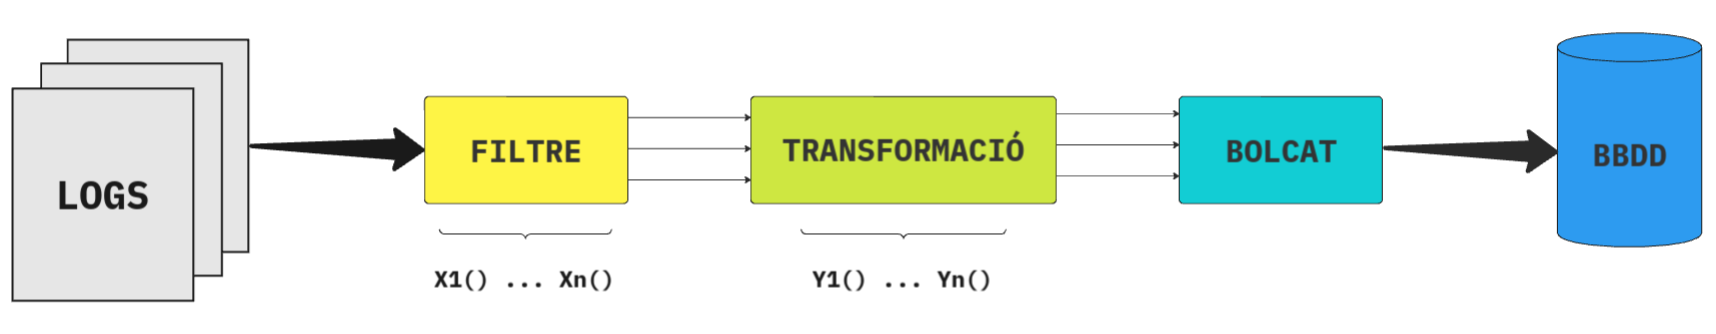
\includegraphics[width=1\textwidth]{figures/log-processing}}
    \captionsetup{justification=centering}
    \caption{Disseny tècnic del processament dels \textit{logs}. (\textbf{Font}: Elaboració pròpia.)}\label{fig:log-processing}
\end{figure}

\noindent
Aquest disseny modular té tres components principals: \\

\noindent
\textbf{Component \texttt{Filtre}} \\

\noindent
El component \texttt{Filtre} s’encarrega de filtrar cada \textit{\gls{log}} mitjançant un criteri específic.
Per exemple:
\begin{itemize}
    \item Si només volem admetre \textit{\gls{log}s} que provenen de dispositius mòbils, definirem una funció filtre que ho faci.
\end{itemize}

\noindent
Les funcions de \texttt{Filtre} poden ser additives, és a dir, un mateix \textit{\gls{log}} pot ser filtrat per diverses funcions.
Si cap filtre és necessari, no es definirà cap. \\

\clearpage

\noindent
\textbf{Component \texttt{Transformació}} \\

\noindent
L’objectiu del component \texttt{Transformació} és modificar el format del \textit{\gls{log}} per afegir o treure camps segons els criteris determinats.
Per exemple:

\begin{itemize}
    \item Podem definir una funció de transformació per canviar del format de la data i hora a un UNIX \textit{\gls{timestamp}}.
    \item Eliminar algun camp que es consideri irrellevant s’hauria de fer mitjançant funcions de transformació.
\end{itemize}

\noindent
Les funcions de \texttt{Transformació} poden ser additives, és a dir, un mateix \textit{\gls{log}} pot ser reformat per diverses funcions.
Si cap transformació és necessària, no es definirà cap. \\

\noindent
\textbf{Component \texttt{Bolcat}} \\

\noindent
Finalment, al component \texttt{Bolcat} arribarà el conjunt de \textit{\gls{log}s} desitjats amb el format escollit.
Ara bé, depenen de la base de dades on es vol fer l’agregació, és possible que s’hagin de fer petits retocs per compatibilitzar amb la base de dades. \\

\noindent
\textbf{Processament}

\noindent \\
Així mateix, si tenim \(X_1\)..\(X_N\) funcions filtre, i \(Y_1\)..\(Y_N\) funcions de transformació, i dos casos d’ús, podem definir el comportament desitjat de la següent manera:

\begin{itemize}
    \item \textbf{Cas d'ús \#1}: processa tots els logs, canvia el format de la data i envia'ls a una base de dades PostgreSQL .
    \begin{itemize}
        \item \texttt{Filtre:} -
        \item \texttt{Transformació:} \(Y_1\)
        \item \texttt{Bolcat:} \texttt{PostgreSQLForwarder}
    \end{itemize}
    \item \textbf{Cas d'ús \#2}: processa només els \textit{\gls{log}s} que accedeixin a recursos UPC, afegeix l’enllaç permanent i guarda-ho a un fitxer pla:
    \begin{itemize}
        \item \texttt{Filtre:} \(X_2\)
        \item \texttt{Transformació:} \(Y_2\)
        \item \texttt{Bolcat:} \texttt{FileSystemForwarder}
    \end{itemize}
\end{itemize}

\noindent
Finalment, enviaríem al codi els casos d’ús: \(CU_1\), \(CU_2\) des d'un fitxer de configuració/codi que faci la feina.

\clearpage

\subsection{Implementació}\label{subsec:log-implementation}

\noindent
\texttt{Filtre}.
La interfície del mòdul filtre requereix que les seves implementacions disposin d'una funció \texttt{filter}.
\begin{center}
    \texttt{function filter(Log) -> bool}
\end{center}
Aquesta ha d'acceptar un \textit{\gls{log}} com a paràmetre explícit, i retornar cert, si i només si aquell registre passa el filtre definit.

\noindent \\
S'han desenvolupat les següents funcions:

\begin{itemize}
    \item \texttt{WebResource}: Detecta si el recurs accedit és un recurs web.
    \item \texttt{SearchResource}: Detecta si és una cerca d’un recurs.
    \item \texttt{AccessResource}: Detecta si el recurs accedit és un recurs d’\gls{UPCommons} a través de l'identificador \gls{handle}.
    \item \texttt{WithIPv6Address}: Detecta si el \textit{\gls{log}} té present l’adreça en versió IPv6.
    \item \texttt{WithoutIpAddress}: Detecta si el \textit{\gls{log}} no té present el camp d'adreça \gls{IP}.
    \item \texttt{AccessResourceBitstream}: Detecta si el recurs accedit és un recurs d’\gls{UPCommons} a través de l'identificador \gls{bitstream} \gls{UUID} .
\end{itemize}

\noindent \\
\texttt{Bolcat}:
\begin{itemize}
    \item \texttt{InfluxDbForwarder}:
    \begin{itemize}
        \item Adaptar el \textit{\gls{log}} en format JSON al format específic de la base de dades.
        \item Enviar el \textit{\gls{log}} a la base de dades.
    \end{itemize}
\end{itemize}

\clearpage

\noindent
\texttt{Transformació}.
La interfície del mòdul filtre requereix que les seves implementacions disposin d'una funció \texttt{transform}.
A causa de la variabilitat d'aquestes funcions, la interfície no exigeix en forma de contracte cap funció.

\noindent \\
S'han desenvolupat les següents funcions:

\noindent \\
\texttt{Transformació}:
\begin{itemize}
    \item \texttt{ToJSON}: Converteix un \textit{\gls{log}} emmagatzemat en una seqüència de caràcters en un \gls{JSON} estructurat.
    \item \texttt{AddLabel}: Afegeix al JSON un parell clau valor.
    \item \texttt{AddTimestamp}: Extrau i afegeix el valor de la data i l'hora.
    \item \texttt{RemoveIPv6Address}: Elimina la adreça \gls{IP} en format IPv6 i manté aquella en format IPv4.
    \item \texttt{AddResourceIdLabel}: Afegeix l'identificador del recurs al qual accedeix el \textit{log}, en cas que aquest sigui un accés a un recurs.
    \item \texttt{AddDefaultIpAddress}: Afegeix una adreça \gls{IP} constant a aquells \textit{\gls{log}s} que no en tinguin cap.
\end{itemize}

\noindent \\
\begin{figure}[htbp]
    \centerline{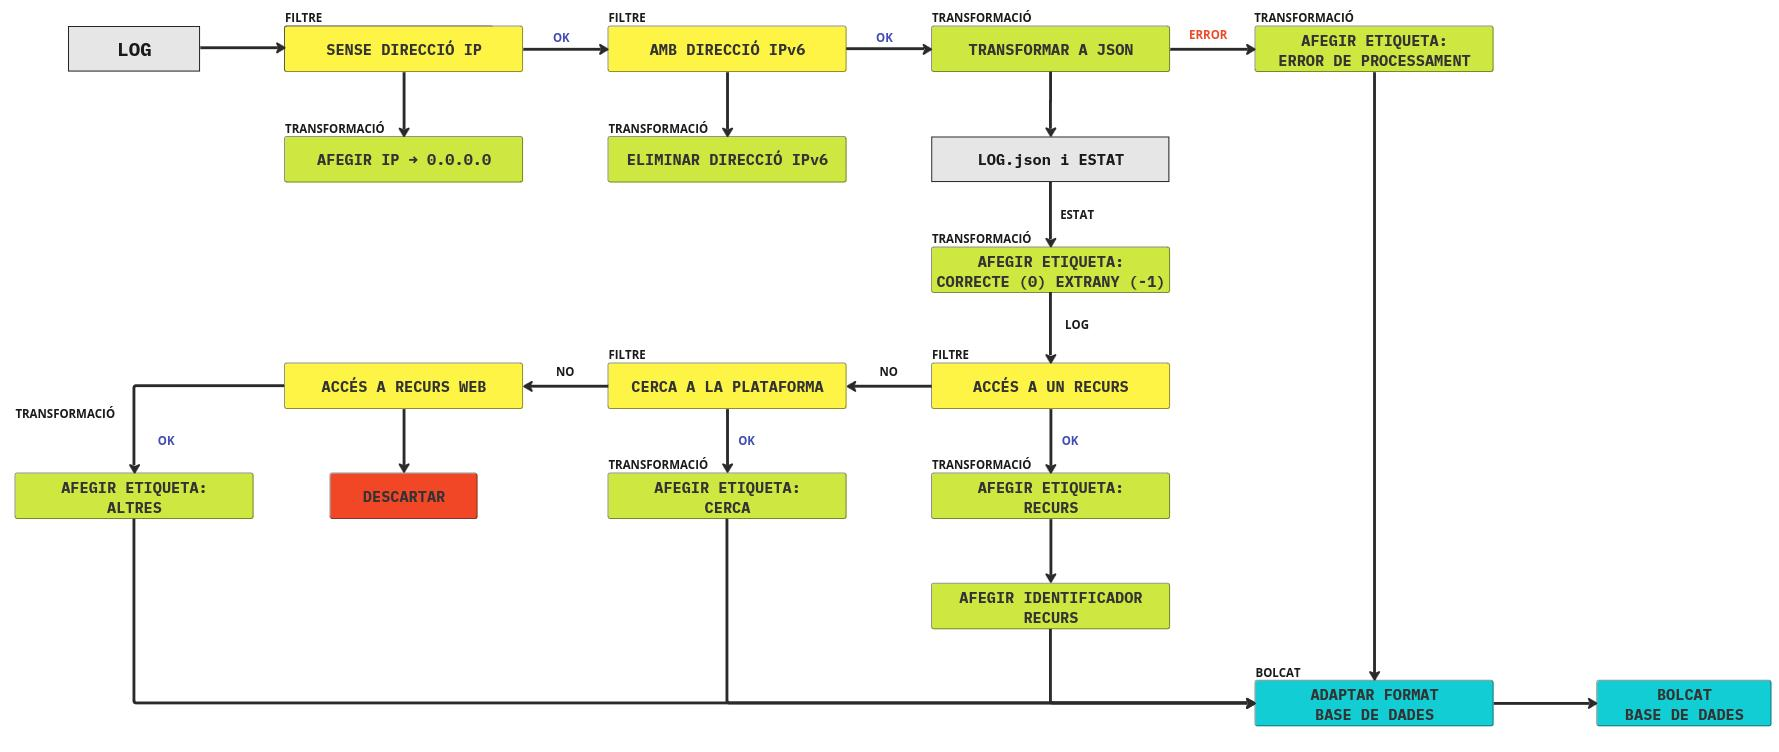
\includegraphics[width=1.3\textwidth]{figures/log-processing-workflow}}
    \captionsetup{justification=centering}
    \caption{Implementació del processament dels \textit{logs}. (\textbf{Font}: Elaboració pròpia.)}\label{fig:log-processing-workflow}
\end{figure}